\documentclass[a4paper,12pt]{scrartcl}

\usepackage[T1]{fontenc}
\usepackage{lmodern}
\usepackage[utf8]{inputenc}
\usepackage[french]{babel}
\usepackage{graphicx}
\usepackage{microtype} 
\usepackage[onehalfspacing]{setspace}
\usepackage[top=2.5cm, bottom=2.5cm, left=3cm, right=3.5cm]{geometry}
\usepackage{tabularx}
\usepackage{graphicx}
\usepackage{longtable}
\usepackage{listings}
\usepackage{listingsutf8}
\usepackage{dsfont}
\usepackage{appendix}
\usepackage{amsmath}
\usepackage{hyperref}
\usepackage{mathtools, amssymb}
\usepackage[usenames,dvipsnames]{color}

% \begin{equation}
% \begin{split}
%     \dbx & =\dbx[3cm] \\
%     & =\dbx
% \end{split}
% \end{equation}

\definecolor{MyDarkGreen}{rgb}{0.0,0.4,0.0}
\lstloadlanguages{Matlab}
\lstset{language=Matlab,                        % Use MATLAB
        frame=single,                           % Single frame around code
        basicstyle=\small\ttfamily,             % Use small true type font
        keywordstyle=[1]\color{Blue}\bfseries,  % MATLAB functions bold and blue
        keywordstyle=[2]\color{Purple},         % MATLAB function arguments purple
        keywordstyle=[3]\color{Blue}\underbar,  % User functions underlined and blue
        identifierstyle=,                       % Nothing special about identifiers
                                                % Comments small dark green courier
        commentstyle=\usefont{T1}{pcr}{m}{sl}\color{MyDarkGreen}\small,
        stringstyle=\color{Purple},             % Strings are purple
        showstringspaces=false,                 % Don't put marks in string spaces
        tabsize=5,                              % 5 spaces per tab
        %
        %%% Put standard MATLAB functions not included in the default
        %%% language here
        morekeywords={xlim,ylim,var,alpha,factorial,poissrnd,normpdf,normcdf},
        %
        %%% Put MATLAB function parameters here
        morekeywords=[2]{on, off, interp},
        %
        %%% Put user defined functions here
        morekeywords=[3]{brownmo},
        %
        morecomment=[l][\color{Blue}]{...},     % Line continuation (...) like blue comment
        numbers=left,                           % Line numbers on left
        firstnumber=1,                          % Line numbers start with line 1
        numberstyle=\tiny\color{Blue},          % Line numbers are blue
        stepnumber=5,                           % Line numbers go in steps of 5
        literate=%                              % accents and Umlaute
                 {Ö}{{\"O}}1
                 {Ä}{{\"A}}1
                 {Ü}{{\"U}}1
                 {ß}{{\ss}}1
                 {ü}{{\"u}}1
                 {ä}{{\"a}}1
                 {ö}{{\"o}}1
                 {\$}{{\dollar}}1
        }

\title{Mini projet 1: Calcul du prix d'une option asiatique}
\author{Valentin DE CRESPIN DE BILLY \\ Matthias LANG}
\date{30.11.2021}

\linespread{1.5} 


\begin{document}

\maketitle
\begin{center}

  \thispagestyle{empty}

  N. d'étudiant: 247067 et 313411\\
  Université Catholique de l'Ouest\\
  Mathématiques financières

\end{center}

\newpage

\section{Calculer le prix du sous-jacent}

Nous avons essayé d'atteindre une équation qui ne dèpend que des variables connues comme la formule de Black-Scholes.
Cela n'a pas fonctionné.

\begin{align}%equation} \label{1} 
dS_t  &=  S_t(rdt+\sigma \sqrt{S_t} dW_t) \\
     \iff \frac{dS_t}{S_t}  &=  rdt+\sigma \sqrt{S_t} dW_t
\end{align}


On prend l'équation 1:
%\begin{equation} \label{3}
%\begin{multlined}
\begin{align*}
= dS_t~=~S_trdt+\sigma S_t^{1.5} dW_t ~~
\text{; Puis} \\
d \langle S_t &, ~ S_t\rangle \\
=\langle dS_t &,~ dS_t\rangle ~=\\
=\langle S_trdt+\sigma S_t^{1.5} dW_t &,~
         S_trdt+\sigma S_t^{1.5} dW_t \rangle ~=\\
=\langle \sigma S_t^{1.5} dW_t &,~
         \sigma S_t^{1.5} dW_t \rangle ~=\\
=S_t^3 \sigma^2 \langle dW_t &,~  dW_t \rangle ~=\\
=S_t^3 \sigma^2 dt
\end{align*}


On pose: 
$X_t = ln(S_t)$
%\begin{equation} \label{4}
%\begin{multlined}
\begin{align}
\text{Formule d'Ito: } dln(S_t) = \frac{dS_t}{S_t} + \frac{1}{2} \frac{-1}{S_t^2}d \langle S_t, ~S_t \rangle \\
\end{align}
Avec les équations 2 et 3:
\begin{align}
dln(S_t) = 
rdt + \sigma \sqrt{S_t} dW_t - \frac{1}{2}S_t \sigma^2 dt =
(r - \frac{1}{2}S_t\sigma^2)dt + \sigma\sqrt{S_t}dW_t
\end{align}


\begin{align*}
ln( \frac{S_t}{S_0} ) 
&= ln(S_t)-ln(S_0) = \int_0^t dln(S_u) = \\
&= \int_0^t (r-\frac{1}{2} S_t \sigma^2)du~+~\int_0^t \sigma \sqrt{S_t}dW_t \\
&=\dots
\end{align*}
Donc on ne peut pas facilement dériver une formule pour le prix comme ça, qui dépend que des variables fixées, mais on peut le simuler pas à pas en utilisant (1):

\begin{equation} \label{6}
\begin{split}
S_0  &~\text{soit connu} \\
dS_0 &= S_0(rdt + \sigma \sqrt{S_0} dW_0) \\
S_1  &\approx S_0 + dS_0 \\
dS_1 &= S_1(rdt + \sigma \sqrt{S_1} dW_1) \\
S_2  &\approx S_1 + dS_1 \\
\dots
\end{split}
\end{equation}


\subsection{ecdf}
Sieht Gaussian aus -> KI damit probieren, aber keine richtige Normalverteilung, also bootstrap!

\subsection{Réduction de la variance du éstimateur}

Les éstimateurs ont une variance telle que:
$ \hat{Var}(C) = \hat{\sigma_i^2} / n_t$, oú $n_t$ est le nombre des observations et $\hat{\sigma_i^2}$ est la variance estimée de la population, qui est égal à la variance de l'échantillon.

Supposons que nous ne connaissions ni les paramètres ni la règle à partir desquels les prix sont établis. 
Nous ne pouvons donc pas augmenter le nombre d'observations pour améliorer l'estimateur.
Quelle autre possibilité existe-t-il pour réduire sa variance ?

Avec les techniques de bootstrap on pourrait répliquer les données. 
Mais on risque de introduir un biais.
Si on utilise une variable de contrôle on n'invente pas des nouvelles données, ni risque-t-on de changer l'ésperance.

% variable antith

\section{Réalisation numerique}

Les algorithmes sont réalisées avec deux langues de programmation: Matlab et Visual Basic for Applications.
Plusieurs graphiques sont y générés, vous les trouverez dans l'annexe \ref{graphiques}.
En plus, avec le logiciel Excel nous avons crée un dashboard, voir une capture d'figure ref{X}. 
Vous trouverez les scriptes et les images dans l'annexe, et avec la fiche de dashboard également dans le \href{https://github.com/matthias-10/UCO_actuariat_mini-projet}{repository}.


\subsection{Variable antithétique}
\subsection{Variables de contrôle}

Afin de réaliser une réduction de variance de l'éstimateur, sans être contraint des ressources de calculation, on peut se servire des variables des contrôle.
Soit $X$ la variable aléatoire dont on veut obtenir l'éstimateur Monte Carlo.
Pour chaque $X_i$ on peut simuler une autre variable $Y_i$, la variable de contrôle.

Cette variable est indépendante, mais correlée avec $X$.
D'ailleurs on sait son ésperance.
Avec les deux valeurs on creer une autre série de données ainsi:
$Z_i = X_i - \lambda(Y_i - E(Y_i))$ avec $\lambda = sigma_X/sigma_Y * \rho$.

\subsubsection{Variable de contrôle 1}

La première variable est construite avec des bruits blancs, plus ou moins la même manière que le prix d'action.
Problematique: Les X et Y ne sont pas independant en utilisant le meme processus?
Non overlapping increments Wt-Ws and Wv-Wu for any 0=s<t=>u<v are independent of each other.
On ajoute $S_0$ pour que les deux puissent être comparées.
$$X_i = S_0 + sum_{i=1}^{n} W_{t_i}$$

C'est facile de démontrer l'ésperance:
$$\mathbb{E}[X_i]=\mathbb{E}[S_0 + sum_{i=1}^{n} W_{t_i}] = S_0$$

La variance, sachant que $\mathbb{E}[W_1*W_2] =\mathbb{E}[W_t_1]*\mathbb{E}[W_t_2] =0$ et $Var(W_t_1) = t_1$, donc  $cov(W_t_1, W_t_2) = t_1$:
$$var(X_i) = 
var(S_0 + sum_{i=1}^{n} W_{t_i}) = 
var(sum_{i=1}^{n} W_{t_i}) = 
\mathbb{E}[(sum_{i=1}^{n} W_{t_i})^2] = 
var(sum_{i=1}^{n} W_{t_i}) =
\sum_{i=1}^n cov(W_t_i, W_t_i) = 
\sum_{i=1}^n \sum_{j=1}^n cov(W_t_i, W_t_i) =
\sum_{i=1}^n \sum_{j=1}^i cov(W_t_i, W_t_j) + sum_{i=1}^{n-1} \sum_{j=i+1}^n cov(W_t_i, W_t_j) =
\sum_{i=1}^n \sum_{j=1}^i t_k + sum_{i=1}^{n-1} \sum_{j=i+1}^n t_i =
T(\sum_{i=1}^n \sum_{j=1}^i \frac{k}{n} + sum_{i=1}^{n-1} \sum_{j=i+1}^n \frac{i}{n}) =
\frac{T}{n}(\sum_{i=1}^n \frac{i(i+1)}{2} + sum_{i=1}^{n-1} i(n-i)) =
\frac{T}{n}(\frac{1}{6}n(n+1)(n+2)+\frac{1}{6}n(n-1)(n+1)) =
\frac{T}{6}(2n^2+3n+1)
$$

Avec cela et on calcule $\lambda$. lambda peut-être calculé avec des données différentes.
De toute façon le temps de calcul de $\lambda$ n'est pris compte dans le temps de calcul affiché.

\subsubsection{Variable de contrôle 2}

Comme deuxième variable de contrôle sert un mouvement brownien des même pas que les trajectoires et avec $W_t_0=S_0$.
Ce-ci suit que son ésperance égal $S_0$ et sa variance $T$.
La covariance doit être calculée empiriquement.
Avec un échantillon de $n=200$ on calcule ainsi le $\lambda$ avant qu'on simule les $Z_i$.
D'où on n'utilize pas trop de calculations, le temps de calcul ne sera pas biais,
et, le plus important, $Z_i$ et $\lambda$ seront indépendant de l'autre.


% si K proche de S_T l'estimateur est trop bas. Pourquoi ?

\subsubsection{Variable de contrôle 3}
En surplus, ces variables ne sont réalisées que en matlab.

C'est pratique de remplacer la variance par sa contrepartie empirique. 

%%%%%%%% A N N E X E %%%%%%%%%%%%%%%%%%
\clearpage

\appendix
\appendixpage
\addappheadtotoc

\begin{center}
Toutes les fiches se trouvent dans le repository en ligne: 

 \url{https://github.com/matthias-10/UCO_actuariat_mini-projet}
\end{center}

\section{Graphiques} \label{graphiques}

\begin{figure}[h!]
  \begin{center}
    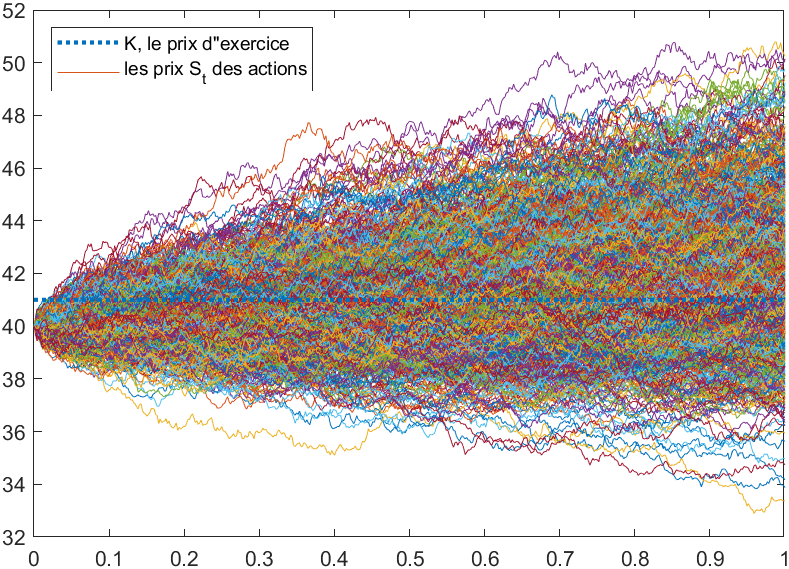
\includegraphics[width=14cm]{"graphiques/S.png"}
    \caption{Les graphes de tous trajectoires, plotés avec matlab}
    \label{fig:S}
  \end{center}
\end{figure}

\begin{figure}[h!]
  \begin{center}
    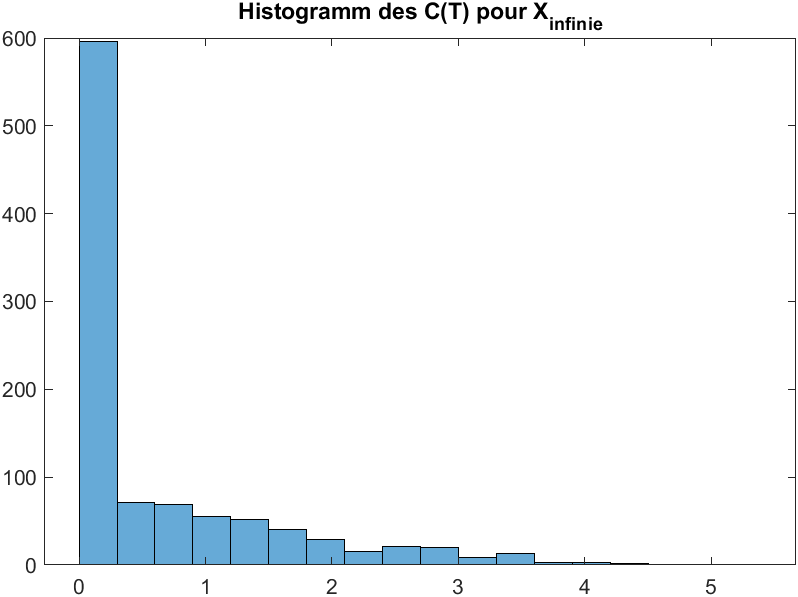
\includegraphics[width=14cm]{"graphiques/hist_C_inf.png"}
    \caption{Histogramme des simulations pour $C_{\infty}$}
    \label{fig:hist_C_inf}
  \end{center}
\end{figure}

\begin{figure}[h!]
  \begin{center}
    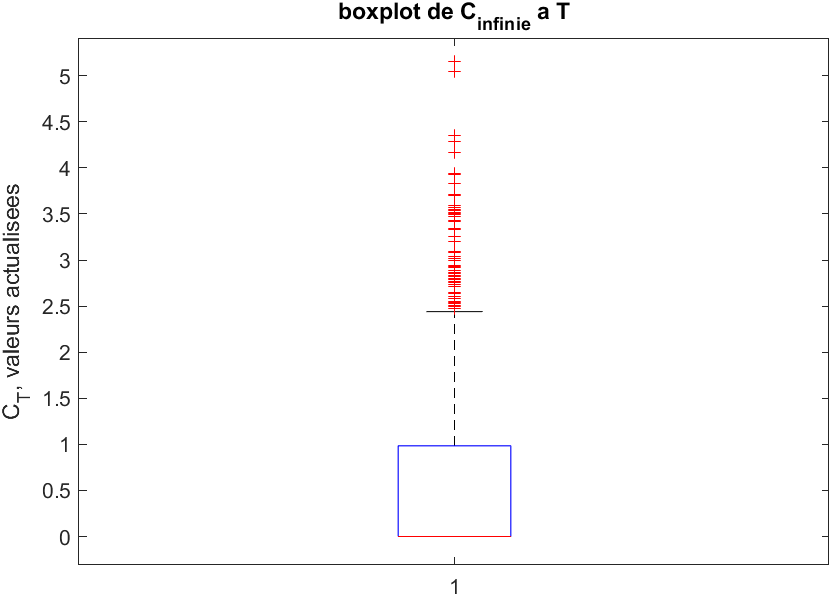
\includegraphics[width=14cm]{"graphiques/box_C_inf.png"}
    \caption{Boxplot des simulations pour $C_{\infty}$}
    \label{fig:box_C_inf}
  \end{center}
\end{figure}

\begin{figure}[h!]
  \begin{center}
    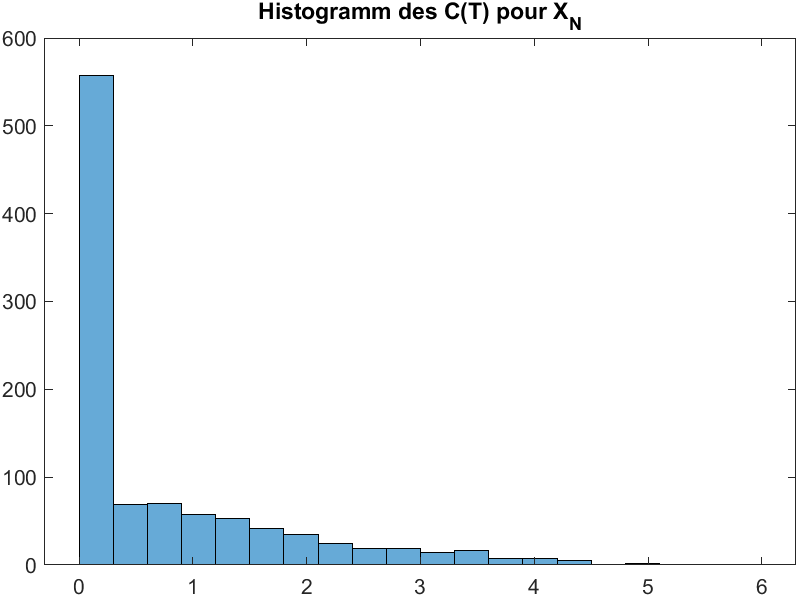
\includegraphics[width=14cm]{"graphiques/hist_C_N.png"}
    \caption{Histogramme des simulations pour $C_{N}$}
    \label{fig:hist_C_N}
  \end{center}
\end{figure}

\begin{figure}[h!]
  \begin{center}
    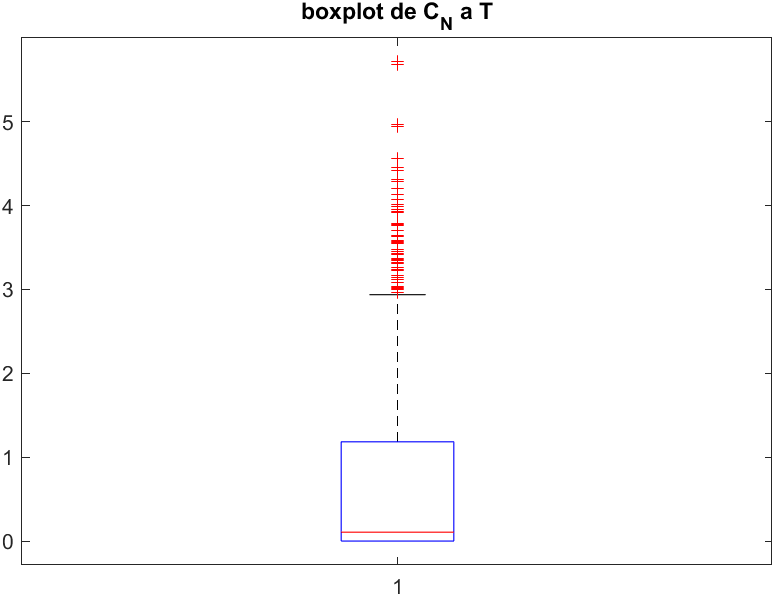
\includegraphics[width=14cm]{"graphiques/box_C_N.png"}
    \caption{Boxplot des simulations pour $C_{N}$}
    \label{fig:box_C_N}
  \end{center}
\end{figure}

\begin{figure}[h!]
  \begin{center}
    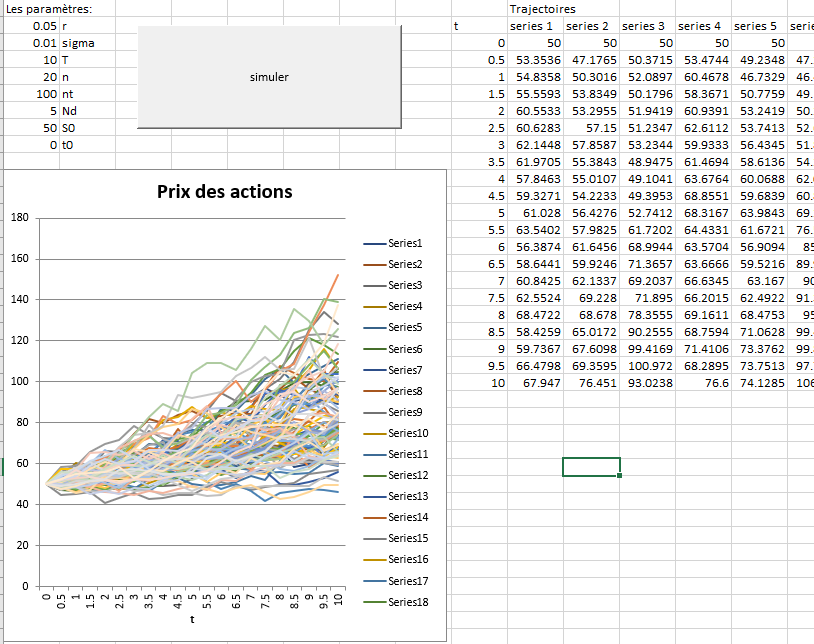
\includegraphics[width=14cm]{"graphiques/Capture.PNG"}
    \caption{le Excel dashboard}
    \label{fig:capture}
  \end{center}
\end{figure}


\section{Code Matlab}
\lstinputlisting{mini_projet.m}

\section{Code VBA}
\lstinputlisting[
    breaklines=true,
    tabsize=3,
    showstringspaces=false
    extendedchars=\true,
    language={[Visual]Basic},
    frame=single,
    framesep=3pt,%expand outward.
    framerule=0.4pt,%expand outward.
    xleftmargin=3.4pt,%make the frame fits in the text area. 
    xrightmargin=3.4pt,%make the frame fits in the text area.
    ]{VBA_script.txt}

\end{document}